% ====================================================================
% Book chapter: extension of the SELENE conference paper.
% Class: Springer Nature official "SNmult" contributed-volume template
% (author/author.tex sample), as supplied by the editor/publisher.
%
% BUILD:
%   tectonic main.tex   (or: pdflatex main && bibtex main && pdflatex main x2)
%
% Figures live in figures/ and are produced by the two experiment
% scripts (see ../book_chapter/). Regenerate with:
%   cp ../book_chapter/outputs/*.pdf figures/
% ====================================================================
\documentclass[graybox]{SNmult}

\usepackage{graphicx}
\usepackage{amsmath,amssymb}
\usepackage{booktabs}
\usepackage{url}

\begin{document}

\title*{Toward Trustworthy Lunar Radiation Nowcasting: Calibrated Uncertainty and Physical Interpretability in Data-Driven Dose-Rate Estimation}
\titlerunning{Trustworthy Lunar Radiation Nowcasting}

\author{Sai Srikar Tummala \and Mittansh Bhatia \and Robert Chun}
\authorrunning{S.\,S. Tummala, M. Bhatia, and R. Chun}

\institute{
  Sai Srikar Tummala \at Independent Researcher, San Jose, CA, USA, \email{tummalasaisrikar@gmail.com}
  \and
  Mittansh Bhatia \at Independent Researcher, Sunnyvale, CA, USA, \email{bhatiamittansh@gmail.com}
  \and
  Robert Chun \at Department of Computer Science, San Jose State University, San Jose, CA, USA, \email{robert.chun@sjsu.edu}
}

\maketitle

\abstract*{Fast, data-driven estimation of the lunar surface radiation environment is now
feasible: in prior work we introduced SELENE, a neural network that predicts
absorbed dose rates from upstream solar and cosmic-ray particle fluxes at a
fraction of the cost of physics-based transport codes~\cite{tummala2025selene}.
Accuracy alone, however, is not sufficient for a model that would inform crew
safety decisions during Artemis-era operations. This chapter argues that an
operationally useful dose-rate model must additionally be \emph{trustworthy}:
it must express calibrated uncertainty and admit a physical interpretation of
its predictions. We extend the SELENE model along both axes. First, we conduct
a physical interpretability and ablation study that attributes the model's
predictions to specific galactic-cosmic-ray and solar-energetic-particle ion
species and energy bands, using permutation importance, Shapley additive
explanations, and a gradient-boosted-tree cross-check, and we quantify how
predictive skill degrades as features are removed. Second, we perform a
calibration analysis of three uncertainty-quantification strategies (Monte
Carlo dropout, deep ensembles, and quantile regression), evaluating each with
reliability diagrams, expected calibration error, and prediction-interval
coverage, and we derive an operational risk-flagging threshold. Together these
analyses convert a fast black-box regressor into an interpretable,
uncertainty-aware nowcasting tool, and we discuss the implications for onboard
deployment and for extension to the Martian radiation environment.
\keywords{lunar radiation $\cdot$ space weather $\cdot$ uncertainty quantification $\cdot$ model calibration $\cdot$ interpretability $\cdot$ deep learning}}

\abstract{Fast, data-driven estimation of the lunar surface radiation environment is now
feasible: in prior work we introduced SELENE, a neural network that predicts
absorbed dose rates from upstream solar and cosmic-ray particle fluxes at a
fraction of the cost of physics-based transport codes~\cite{tummala2025selene}.
Accuracy alone, however, is not sufficient for a model that would inform crew
safety decisions during Artemis-era operations. This chapter argues that an
operationally useful dose-rate model must additionally be \emph{trustworthy}:
it must express calibrated uncertainty and admit a physical interpretation of
its predictions. We extend the SELENE model along both axes. First, we conduct
a physical interpretability and ablation study that attributes the model's
predictions to specific galactic-cosmic-ray and solar-energetic-particle ion
species and energy bands, using permutation importance, Shapley additive
explanations, and a gradient-boosted-tree cross-check, and we quantify how
predictive skill degrades as features are removed. Second, we perform a
calibration analysis of three uncertainty-quantification strategies (Monte
Carlo dropout, deep ensembles, and quantile regression), evaluating each with
reliability diagrams, expected calibration error, and prediction-interval
coverage, and we derive an operational risk-flagging threshold. Together these
analyses convert a fast black-box regressor into an interpretable,
uncertainty-aware nowcasting tool, and we discuss the implications for onboard
deployment and for extension to the Martian radiation environment.
\keywords{lunar radiation $\cdot$ space weather $\cdot$ uncertainty quantification $\cdot$ model calibration $\cdot$ interpretability $\cdot$ deep learning}}

% ====================================================================
\section{Introduction}
\label{sec:intro}

Sustained human presence on the Moon, envisioned by NASA's Artemis
program~\cite{artemis2020plan}, requires accurate, timely knowledge of the
surface radiation environment. Unlike Earth, the Moon has neither a global
magnetic field nor a substantial atmosphere, so its surface is continuously
exposed to galactic cosmic rays (GCRs) and, episodically, to intense solar
energetic particle (SEP) events. The resulting absorbed dose poses acute and
long-term risks to astronauts and can disrupt
electronics~\cite{durante2011physical,cucinotta2014space}. Mission planners need
dose estimates that are
both fast enough for operational timescales and reliable enough to act upon.

Physics-based transport codes such as HZETRN and Monte Carlo tools such as
GEANT4 remain the gold standard for radiation
modeling~\cite{Slaba2013,Singleterry2010,2022cosp...44.2697D}, but their computational cost and their
dependence on detailed shielding and geometry inputs make them awkward for
real-time, resource-constrained decision-making. In prior
work~\cite{tummala2025selene} we proposed a complementary, data-driven approach:
SELENE (Space Environment Lunar Exposure Neural Estimator), a feedforward neural
network that learns the mapping from upstream particle-flux measurements made by
the Advanced Composition Explorer (ACE) to the absorbed dose rate measured at
the Moon by the Cosmic Ray Telescope for the Effects of Radiation
(CRaTER)~\cite{Spence2010,Looper2020}. SELENE demonstrated that machine learning
can approximate the dose response quickly and with useful accuracy.

Accuracy, however, is a necessary but not a sufficient condition for
operational adoption. A model that would inform crew safety decisions must also
answer two further questions: \emph{how confident is this prediction?} and
\emph{why did the model produce it?} A point estimate with no uncertainty gives
an operator no basis for deciding when to seek shelter or defer an activity; and
an unexplained estimate is difficult to trust, audit, or reconcile with physical
expectations. These twin requirements, calibrated uncertainty and physical
interpretability, are the subject of this chapter.

We make two contributions that extend SELENE from a fast regressor into a
trustworthy nowcasting tool:
\begin{enumerate}
  \item A \emph{physical interpretability and ablation} study
        (Sect.~\ref{sec:interp}) that identifies which GCR and SEP ion species
        and energy bands drive the model's dose predictions, and quantifies how
        predictive skill responds as informative features are removed.
  \item A \emph{calibration} study (Sect.~\ref{sec:calib}) that compares three
        uncertainty-quantification strategies and derives an operational
        risk-flagging threshold from the best-calibrated method.
\end{enumerate}

The remainder of the chapter is organized as follows.
Sect.~\ref{sec:background} reviews the physics of the lunar radiation
environment and the instrumentation used. Sect.~\ref{sec:related} surveys
physics-based and data-driven modeling and situates our contributions within the
literature on uncertainty quantification and interpretability.
Sect.~\ref{sec:selene} recaps the SELENE model~\cite{tummala2025selene}.
Sects.~\ref{sec:interp} and~\ref{sec:calib} present the two new studies.
Sect.~\ref{sec:discussion} discusses operational implications and limitations,
and Sect.~\ref{sec:conclusion} concludes.

% ====================================================================
\section{Background: The Lunar Radiation Environment}
\label{sec:background}

\subsection{Sources of Radiation}
Two populations dominate the charged-particle radiation reaching the lunar
surface. \emph{Galactic cosmic rays} are high-energy nuclei originating outside
the solar system, composed mostly of protons and helium with a small but
biologically important heavy-ion component; their flux is anticorrelated with
solar activity over the roughly 11-year solar cycle. \emph{Solar energetic
particles} are emitted sporadically during solar flares and coronal mass
ejections, producing sudden, order-of-magnitude enhancements in particle flux
over minutes to days~\cite{durante2011physical}. Because the Moon lacks a
magnetosphere, both populations reach the surface essentially unimpeded, and
secondary particles (including albedo neutrons) are generated in the
regolith~\cite{Zhang2020,Wimmer2020}.

\subsection{Dosimetric Quantities}
Radiation exposure is described by several related quantities. The
\emph{absorbed dose} $D$ is the energy deposited per unit mass, measured in gray
($1~\mathrm{Gy} = 1~\mathrm{J/kg}$); our target variable is a daily absorbed
dose rate. The biological impact of a given absorbed dose depends on the
particle type and energy, captured by the \emph{linear energy transfer} (LET),
the energy deposited per unit path length. The \emph{dose equivalent} $H = Q\,D$
weights the absorbed dose by a quality factor $Q$ that increases with LET, so
that densely ionizing heavy ions are penalized relative to sparsely ionizing
protons~\cite{durante2011physical,cucinotta2014space}. Long-term GCR LET spectra
in lunar orbit have been characterized directly by
CRaTER~\cite{Looper2020,schwadron2012lunar}. In this chapter we model the absorbed dose rate directly and
treat quality-factor weighting as a downstream transformation.

\subsection{Instrumentation}
Our data combine two spaceborne assets. CRaTER, aboard the Lunar Reconnaissance
Orbiter, measures the dose rate and LET spectrum in lunar orbit and provides the
prediction target~\cite{Spence2010,schwadron2012lunar}. ACE, stationed at the
Sun--Earth L1 point since 1997, provides the upstream predictors: its Cosmic Ray
Isotope Spectrometer (CRIS) resolves GCR heavy-ion
composition~\cite{Cummings1998,Stone1998ACE}, and its Solar Isotope Spectrometer (SIS) measures SEP fluxes
during solar events~\cite{Stone1998SIS}. Because ACE observes the particle
environment upstream of the Earth--Moon system, its measurements carry
predictive information about the dose subsequently recorded at the Moon.

\subsection{Career Dose Limits and Operational Thresholds}
The dosimetric quantities defined above are not merely descriptive; they anchor
concrete operational limits. NASA's permissible exposure limits bound an
astronaut's career effective dose to keep the resulting increase in lifetime
cancer risk below a fixed threshold, with the exact numerical limit depending on
age and sex because of differences in latency and background
risk~\cite{cucinotta2014space}. Because GCR dose accrues continuously while SEP
events can deliver a substantial fraction of a mission's total dose in hours to
days, operational risk management in practice reduces to two decisions: how much
of the career limit a given mission may consume, and when, during an SEP event,
the instantaneous dose \emph{rate} is high enough to warrant sheltering behind
additional mass shielding~\cite{durante2011physical}. A dose-rate model that will
inform either decision must therefore be evaluated not only on average accuracy
but specifically on its behavior during the high-dose-rate tail that dominates
career-limit consumption and shelter decisions, a point we return to
quantitatively in Sects.~\ref{sec:calib} and~\ref{sec:discussion}.

% ====================================================================
\section{Related Work}
\label{sec:related}

\subsection{Physics-Based Modeling and Dosimetry}
Deterministic and Monte Carlo transport codes are the established tools for
space-radiation modeling. HZETRN provides fast deterministic heavy-ion
transport~\cite{Slaba2013}; OLTARIS packages such capabilities for mission
analysis~\cite{Singleterry2010}; and REDMoon applies GEANT4 Monte Carlo
simulation specifically to the lunar surface and subsurface~\cite{2022cosp...44.2697D}.
These approaches are physically faithful but computationally heavy and demand
detailed geometry and shielding inputs. Direct dosimetry provides ground truth:
the Lunar Lander Neutron and Dosimetry experiment on Chang'e~4 delivered the
first surface dose measurements~\cite{Wimmer2020,Zhang2020}, complementing the
long-term orbital record from CRaTER~\cite{Looper2020,schwadron2012lunar}.

\subsection{Data-Driven Forecasting}
Machine learning has been applied primarily to \emph{forecasting} space-weather
drivers rather than to estimating absorbed dose. Recurrent networks have been
used to forecast solar proton fluxes~\cite{Papagiannopoulos2023}, deep models to
forecast GCR spectra~\cite{Du2024}, and probabilistic models to forecast
radiation exposure for spaceflight~\cite{Zampieri2024}. Our prior
work~\cite{tummala2025selene} differs in target and framing: it learns the dose
\emph{response} to measured fluxes, providing a fast surrogate for transport
calculations. For the tabular regression setting we also benchmark against
gradient-boosted trees~\cite{chen2016xgboost}, random forests~\cite{breiman2001random},
and attention-based tabular transformers~\cite{somepalli2021saint}, following
standard practice~\cite{bishop2006pattern}.

\subsection{Model Capacity and Small, Noisy Tabular Data}
A recurring theme in this literature, and one directly relevant to the present
chapter, is that model capacity must be matched to sample size and signal
strength. Our prior work found that a SAINT transformer, despite being the most
expressive architecture evaluated, performed far worse than the compact SELENE
network on this task, essentially collapsing to a constant
predictor~\cite{tummala2025selene}. This is consistent with a broader pattern in
the tabular deep-learning literature: high-capacity attention-based architectures
are prone to overfitting or to failing to find a useful optimum on datasets of a
few thousand to tens of thousands of rows with a low signal-to-noise ratio,
whereas compact networks with strong regularization, and even simple statistical
baselines~\cite{breiman2001random,bishop2006pattern}, remain competitive or
superior. This motivates two of the design choices in the present chapter: we
retain SELENE's compact architecture rather than scaling it up, and, in
Sect.~\ref{sec:interp}, we ask directly whether the model needs all 18 input
features or whether a smaller, better-matched input space would serve equally
well.

\subsection{Uncertainty Quantification and Interpretability in Scientific ML}
The trustworthiness of scientific machine-learning models has become a research
focus in its own right. Monte Carlo dropout casts dropout as approximate
Bayesian inference to obtain predictive uncertainty~\cite{gal2016dropout}, while
deep ensembles provide a simple, strong alternative~\cite{lakshminarayanan2017ensembles}.
Neural networks are, however, frequently miscalibrated~\cite{guo2017calibration},
motivating explicit calibration analysis and, for regression, calibrated
prediction intervals~\cite{kuleshov2018calibrated}. Quantile
regression~\cite{koenker1978regression} and pinball-loss networks provide
distribution-free intervals and are widely used for probabilistic
forecasting~\cite{rasp2018neural}. On the interpretability side, Shapley additive
explanations offer a unified, theoretically grounded attribution
method~\cite{lundberg2017shap}. To our knowledge, these tools have not previously
been brought together to make a lunar dose-rate model both interpretable and
calibrated; that integration is the contribution of this chapter.

% ====================================================================
\section{The SELENE Model: A Recap}
\label{sec:selene}

This section briefly recaps the model introduced in our prior
work~\cite{tummala2025selene}; readers are referred there for full detail. All
results and design choices in this section are attributable to that paper except
where we note reproduced values.

\paragraph{Data.}
The target is the daily absorbed dose rate recorded by CRaTER. Predictors are
per-day aggregated GCR and SEP ion counts from ACE CRIS and SIS. Because CRaTER
dose was reported daily while ACE fluxes were hourly, all series were harmonized
to a common daily resolution; this temporal alignment was essential, raising the
strongest feature--target correlation from weak to
moderate~\cite{tummala2025selene}. After correlation-based selection, 18 ion/
energy-band features were retained.

\subsection{Dataset Summary Statistics}
\label{sec:dataset-stats}
For this chapter we recomputed dataset statistics directly from the same daily-
aggregated pipeline, both to document the data precisely and to verify the
pipeline before running the two new studies. Table~\ref{tab:dataset} summarizes
the resulting sample sizes and target statistics.

\begin{table}[t]
  \caption{Dataset summary statistics after preprocessing (daily aggregation,
  correlation-based feature selection, and removal of missing/negative rows).
  Dose rate is in Gy/day.}
  \label{tab:dataset}
  \begin{tabular}{p{5.5cm}p{2.5cm}}
    \hline\noalign{\smallskip}
    Quantity & Value \\
    \noalign{\smallskip}\svhline\noalign{\smallskip}
    Total samples ($n$) & 27{,}031 \\
    Training samples & 24{,}327 \\
    Validation samples & 2{,}704 \\
    Input features & 18 \\
    Dose rate: mean & $0.01586$ \\
    Dose rate: median & $0.00978$ \\
    Dose rate: std.\ dev. & $0.04530$ \\
    Dose rate: minimum & $0.0$ \\
    Dose rate: maximum & $1.703$ \\
    \noalign{\smallskip}\hline
  \end{tabular}
\end{table}

The gap between the median ($0.00978$) and the mean ($0.01586$), together with a
maximum roughly $175\times$ the median, indicates a strongly right-skewed,
heavy-tailed distribution. Figure~\ref{fig:target-dist} confirms this directly:
the overwhelming majority of days have near-zero dose rate, with a long tail of
rare days (corresponding to SEP events) reaching dose rates up to two orders
of magnitude higher. This heavy tail is the direct cause of the high-dose
prediction difficulty noted in the original error
analysis~\cite{tummala2025selene} and revisited quantitatively in
Sect.~\ref{sec:calib}.

\begin{figure}[t]
  \centering
  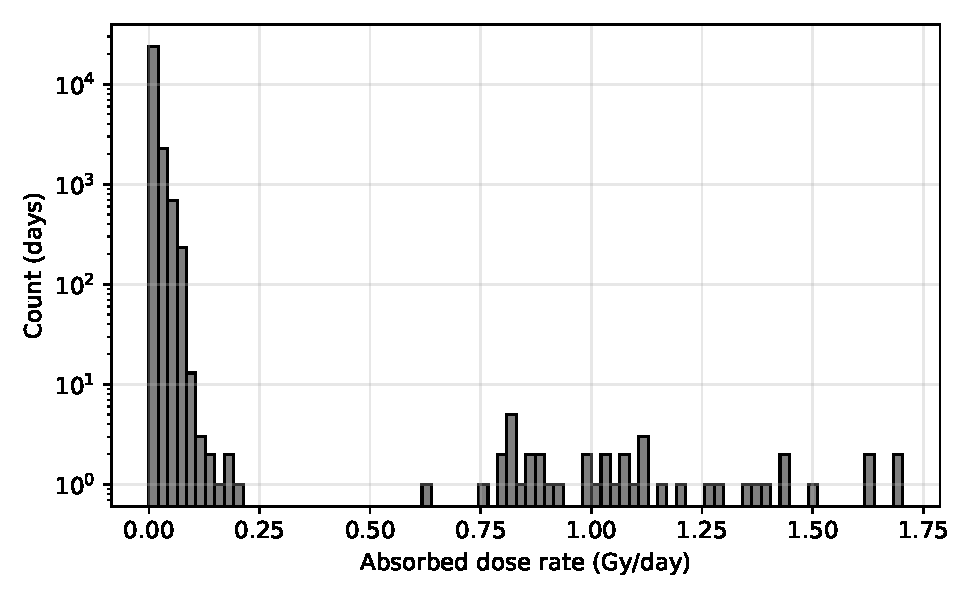
\includegraphics[width=0.68\textwidth]{figures/fig_target_distribution.pdf}
  \Description{Histogram, log-scaled vertical axis, of the daily absorbed dose
  rate across 27,031 samples. The overwhelming majority of samples cluster near
  zero dose rate, with a sparse, long tail of rare samples extending out to
  roughly 1.7 gray per day.}
  \caption{Distribution of the daily absorbed dose rate target across all
  27{,}031 samples (log-scaled count axis to make the heavy tail visible). The
  distribution is dominated by near-zero, quiescent days, with a long tail of
  rare high-dose days driven by SEP events.}
  \label{fig:target-dist}
\end{figure}

\subsection{Feature--Target Correlation}
\label{sec:correlation}
As an independent, model-free check on the feature-selection process described
in the original paper~\cite{tummala2025selene}, we recomputed the raw Pearson
correlation coefficient between each of the 18 retained features and the dose
target. Figure~\ref{fig:raw-corr} shows the result: \texttt{sis\_cnt\_O\_1}
($r = 0.856$), \texttt{sis\_cnt\_O\_2}
($r = 0.853$), and \texttt{sis\_cnt\_C\_2} ($r = 0.845$) are strongly and
positively correlated with dose, while every other feature has $|r| < 0.03$,
statistically indistinguishable from no linear relationship at this sample size.
This simple, model-free statistic already anticipates the more sophisticated
interpretability findings of Sect.~\ref{sec:interp}: three SEP channels carry
essentially all of the linear signal in the dataset, well before any model is
trained.

\begin{figure}[t]
  \centering
  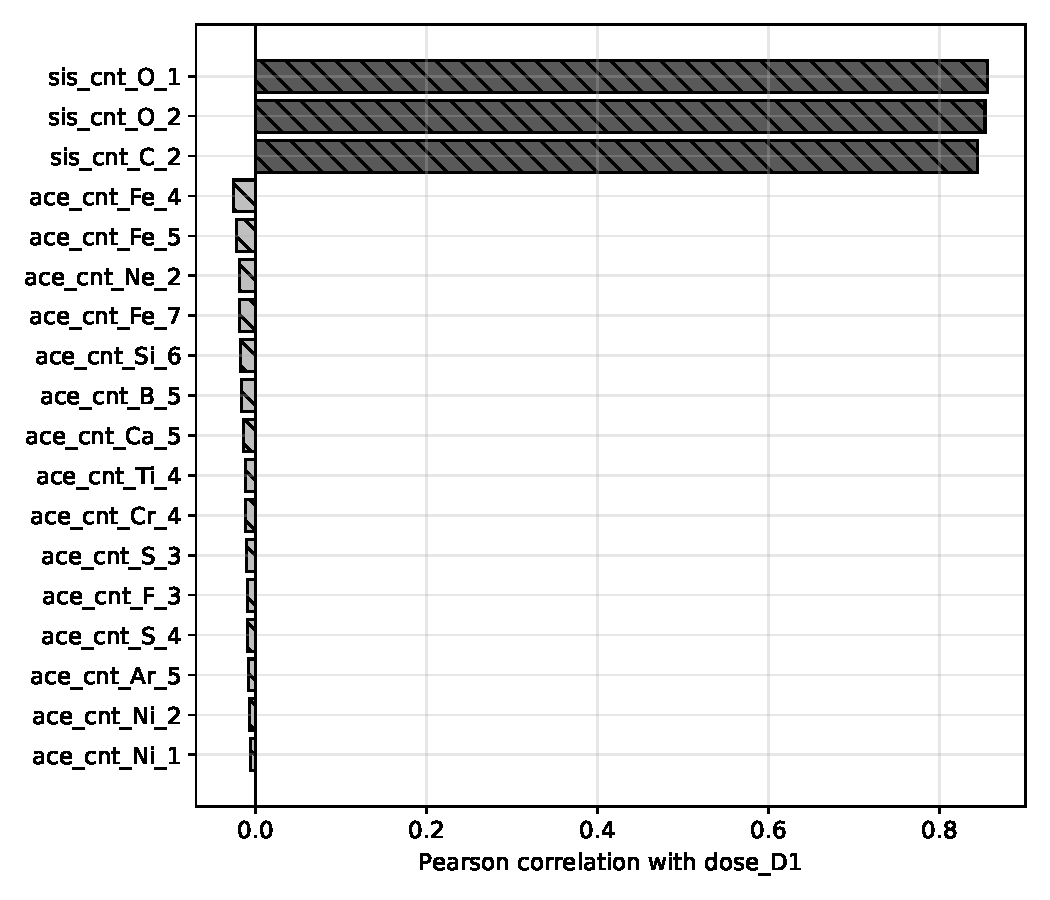
\includegraphics[width=0.7\textwidth]{figures/fig_raw_correlation.pdf}
  \Description{Horizontal bar chart of the Pearson correlation coefficient
  between each of 18 input features and the dose target. Three bars,
  corresponding to solar-energetic-particle carbon and oxygen counts, extend to
  roughly 0.85; the remaining fifteen bars, corresponding to galactic-cosmic-ray
  channels, are close to zero.}
  \caption{Raw Pearson correlation between each of the 18 SELENE input features
  and the dose-rate target. Three SEP features (dark bars) are strongly
  correlated; all GCR features (light bars) are effectively uncorrelated.}
  \label{fig:raw-corr}
\end{figure}

\paragraph{Architecture.}
SELENE is a compact feedforward network: an input layer of 18 features, two
hidden layers of 64 and 32 units with batch normalization, LeakyReLU
activations, and dropout ($0.4$ and $0.3$ respectively), $L_2$ weight
regularization, and a single linear output. It is trained with the Adam
optimizer under a mean-absolute-error loss with early stopping and
learning-rate reduction on plateau~\cite{tummala2025selene}.

\subsection{Evaluation Metrics}
\label{sec:metrics}
We report four standard regression metrics throughout the chapter, evaluated on
the held-out validation set of $n_v$ samples with true values $y_i$ and
predictions $\hat{y}_i$. Mean squared error and mean absolute error,
\begin{equation}
  \mathrm{MSE} = \frac{1}{n_v}\sum_{i=1}^{n_v} (y_i - \hat{y}_i)^2,
  \qquad
  \mathrm{MAE} = \frac{1}{n_v}\sum_{i=1}^{n_v} \lvert y_i - \hat{y}_i \rvert,
  \label{eq:mse-mae}
\end{equation}
penalize large and typical errors respectively. The coefficient of
determination,
\begin{equation}
  R^2 = 1 - \frac{\sum_{i=1}^{n_v} (y_i - \hat{y}_i)^2}
                 {\sum_{i=1}^{n_v} (y_i - \bar{y})^2},
  \qquad \bar{y} = \frac{1}{n_v}\sum_{i=1}^{n_v} y_i,
  \label{eq:r2}
\end{equation}
measures the fraction of target variance explained by the model relative to a
constant-mean baseline; $R^2 = 1$ is a perfect fit and $R^2 \le 0$ means the
model is no better than (or worse than) predicting the mean. Mean absolute
percentage error,
\begin{equation}
  \mathrm{MAPE} = \frac{100\%}{n_v}\sum_{i=1}^{n_v}
    \left\lvert \frac{y_i - \hat{y}_i}{y_i} \right\rvert,
  \label{eq:mape}
\end{equation}
expresses error relative to the magnitude of the target, which is informative
here precisely because the target spans several orders of magnitude
(Table~\ref{tab:dataset}); we clip $|y_i|$ away from zero to avoid division
instability on quiescent days.

\paragraph{Reported and reproduced performance.}
In the original paper SELENE attained a validation coefficient of determination
$R^2 = 0.834$ and a mean absolute percentage error of $14.26\%$, outperforming
linear regression, gradient-boosted trees, and an attention-based tabular
transformer on this noisy dataset~\cite{tummala2025selene}. For the present study
we reproduced the model from the same pipeline; the reproduced validation
metrics were $R^2 = 0.799$ and $\mathrm{MAPE} = 17.45\%$,
consistent with the originally reported values up to the run-to-run variation
expected from stochastic training. The remainder of the chapter analyses this
reproduced model.

% ====================================================================
\section{Physical Interpretability and Ablation}
\label{sec:interp}

A dose-rate model is more trustworthy if the features it relies on agree with
radiation physics. In this section we attribute SELENE's predictions to
individual ion/energy-band features and test how predictive skill depends on
them.

\subsection{Method}
We use three complementary lenses. \emph{Permutation importance} measures the
drop in validation $R^2$ when a single feature's values are randomly shuffled,
breaking its relationship with the target while preserving its marginal
distribution. Formally, for feature $j$ and $R$ independent shuffles,
\begin{equation}
  \mathrm{PI}_j = R^2(f, X) - \frac{1}{R}\sum_{r=1}^{R} R^2\bigl(f, X^{(j,r)}_{\text{perm}}\bigr),
  \label{eq:perm-importance}
\end{equation}
where $R^2(f, X)$ is the model's validation $R^2$ on the unmodified data and
$X^{(j,r)}_{\text{perm}}$ is the validation set with column $j$ independently
shuffled on repeat $r$ (we use $R=20$); features whose permutation most
degrades skill are the most relied-upon.

\emph{Shapley additive explanations} (SHAP) attribute each prediction to its
features using a game-theoretic allocation that is locally accurate and
consistent~\cite{lundberg2017shap}. For feature $j$, sample $x$, and the set of
all features $\mathcal{F}$, the Shapley value is
\begin{equation}
  \phi_j(x) = \sum_{S \subseteq \mathcal{F}\setminus\{j\}}
    \frac{|S|!\,(|\mathcal{F}|-|S|-1)!}{|\mathcal{F}|!}
    \Bigl[f_x(S \cup \{j\}) - f_x(S)\Bigr],
  \label{eq:shap}
\end{equation}
where $f_x(S)$ is the model's expected prediction given only the features in
subset $S$ (the rest marginalized out via the background sample) and the sum
runs over every subset of the remaining $17$ features; $\phi_j(x)$ is feature
$j$'s fair share of the difference between the prediction for $x$ and the
average prediction, averaged over every possible order in which features could
be revealed. Averaging $|\phi_j(x)|$ across validation samples yields the
global importance ranking reported in Table~\ref{tab:attribution}. Because the
$2^{17}$ subsets in Eq.~\ref{eq:shap} are intractable to enumerate exactly,
we use \texttt{KernelExplainer}'s sampling-based approximation with a
$100$-row background sample.

Finally, as a model-agnostic cross-check, we fit a gradient-boosted-tree
regressor~\cite{chen2016xgboost} and compare its gain-based feature importances
with the neural-network attributions. To test dependence on feature count, we
retrain SELENE on the top-$k$ permutation features for
$k \in \{2,4,8,12,18\}$ and record validation skill.

\subsection{Results}
Figure~\ref{fig:perm} shows the permutation-importance ranking. The most
influential predictors were \texttt{sis\_cnt\_C\_2} (mean $R^2$ drop $0.358$),
\texttt{sis\_cnt\_O\_2} ($0.204$), and \texttt{sis\_cnt\_O\_1} ($0.010$),
indicating that the model's skill rests overwhelmingly on SIS-measured SEP
carbon and oxygen counts rather than on the GCR channels from CRIS. The SHAP
summary (Figure~\ref{fig:shap}) yields a consistent ordering, with mean absolute
SHAP values largest for the same three features, \texttt{sis\_cnt\_C\_2}
($0.0133$), \texttt{sis\_cnt\_O\_2} ($0.0105$), and \texttt{sis\_cnt\_O\_1}
($0.0041$). The gradient-boosted-tree cross-check (Figure~\ref{fig:xgb}) agrees
that \texttt{sis\_cnt\_C\_2} is the single most important feature (gain
$0.386$), corroborating the neural attributions, but it assigns substantially
more weight to \texttt{ace\_cnt\_Ca\_5} (gain $0.207$) and \texttt{ace\_cnt\_Fe\_4}
($0.137$) than either permutation importance or SHAP do, a discrepancy we
return to below.

\begin{figure}[t]
  \centering
  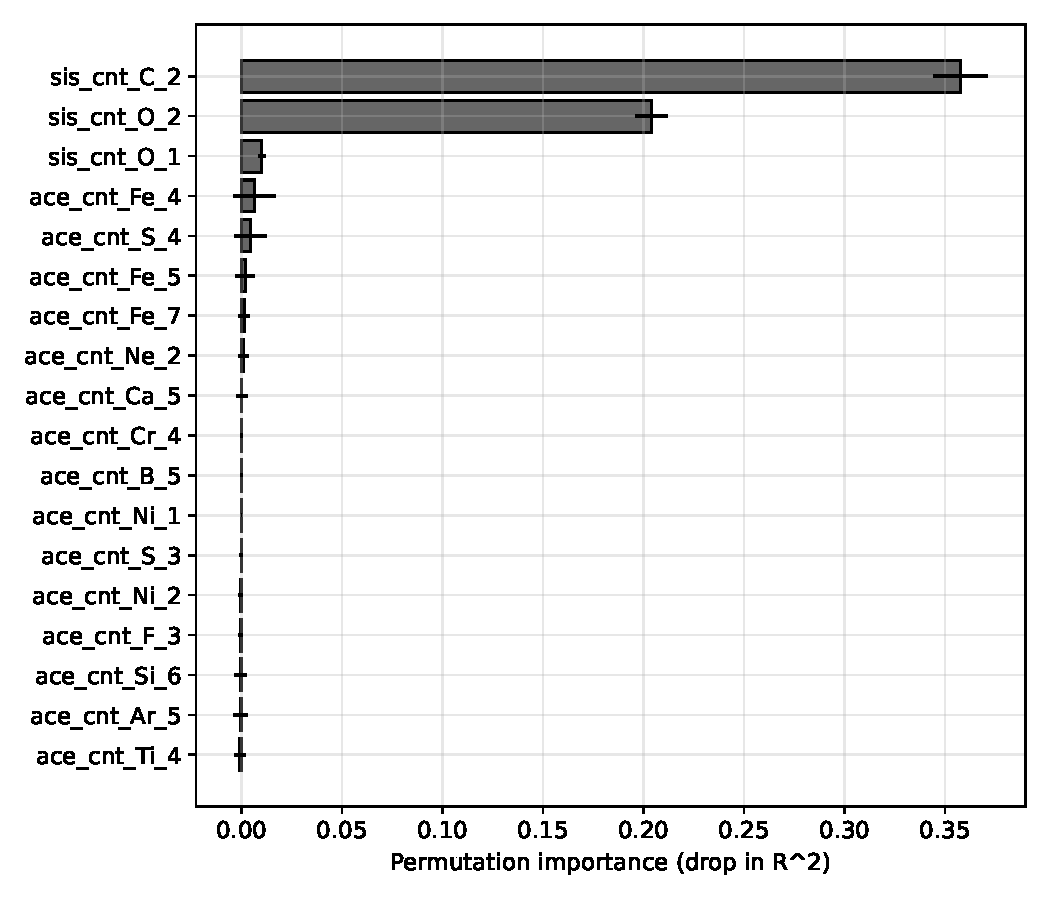
\includegraphics[width=0.72\textwidth]{figures/fig_permutation_importance.pdf}
  \Description{Horizontal bar chart of permutation importance for 18 features.
  Two bars, for solar carbon and oxygen counts, are far longer than the
  remaining sixteen, which cluster near zero.}
  \caption{Permutation importance of the 18 SELENE input features, measured as
  the drop in validation $R^2$ when each feature is shuffled (error bars: standard
  deviation over 20 repeats). Larger values indicate greater reliance.}
  \label{fig:perm}
\end{figure}

\begin{figure}[t]
  \centering
  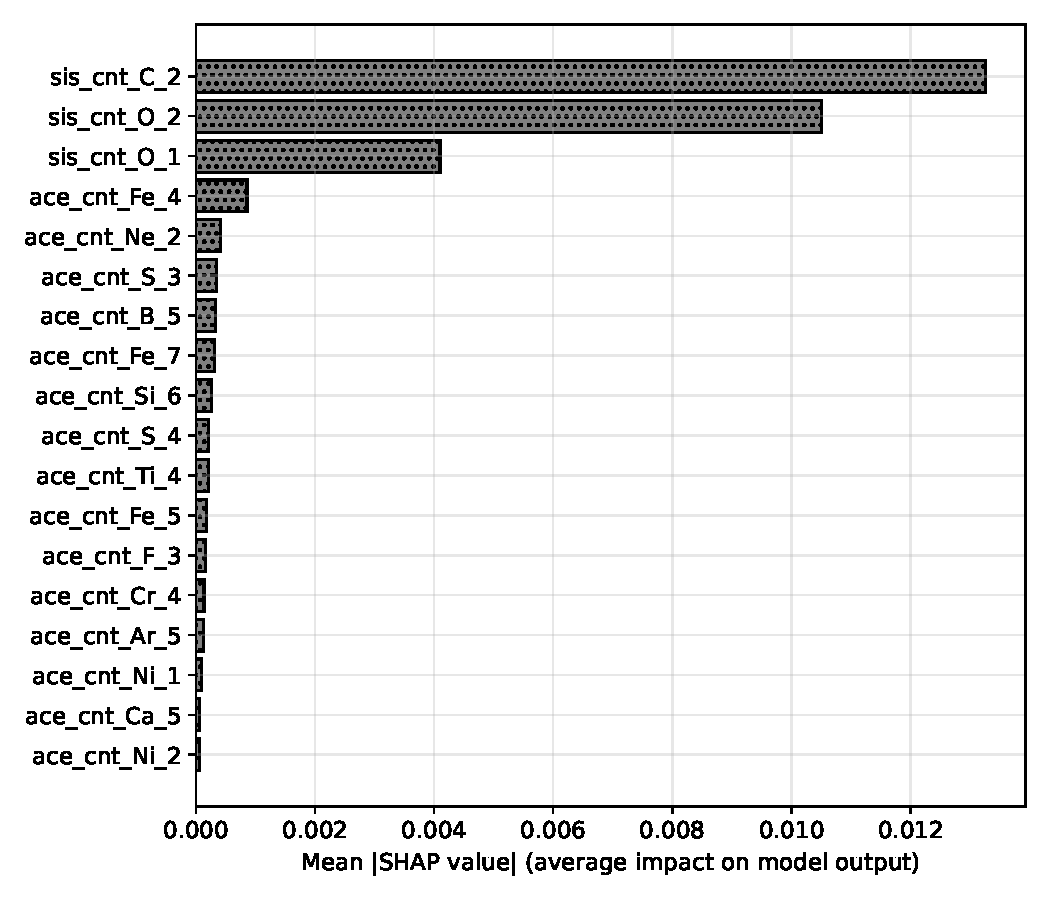
\includegraphics[width=0.72\textwidth]{figures/fig_shap_summary.pdf}
  \Description{Horizontal bar chart of mean absolute SHAP value for 18
  features, ordered by magnitude. The same three solar-particle features
  dominate, matching the permutation-importance ranking.}
  \caption{Mean absolute SHAP value per feature, averaged over 200 validation
  samples. Bars are ordered by magnitude; larger values indicate a feature
  contributed more, on average, to individual predictions.}
  \label{fig:shap}
\end{figure}

\begin{figure}[t]
  \centering
  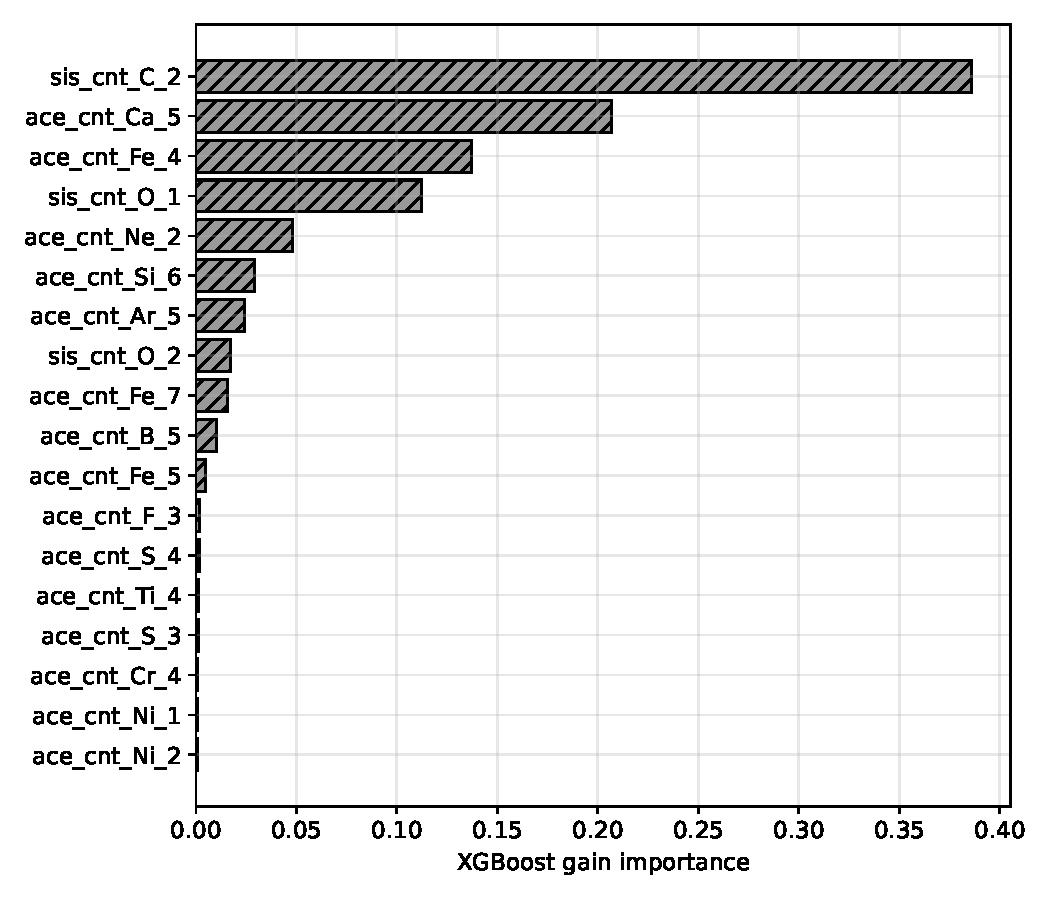
\includegraphics[width=0.72\textwidth]{figures/fig_xgb_importance.pdf}
  \Description{Horizontal bar chart of gain-based feature importance from a
  gradient-boosted-tree model. The top feature matches the neural-network
  attributions, but two galactic-cosmic-ray features receive noticeably higher
  importance than in the other two methods.}
  \caption{Gain-based feature importance from a gradient-boosted-tree
  regressor~\cite{chen2016xgboost}, used as a model-agnostic cross-check on the
  neural-network attributions.}
  \label{fig:xgb}
\end{figure}

Table~\ref{tab:attribution} consolidates all three attribution methods for all
18 features, ordered by permutation importance. The three SEP features occupy
the top three permutation-importance and SHAP ranks; the one clear disagreement
is XGBoost's high gain for \texttt{ace\_cnt\_Ca\_5} and \texttt{ace\_cnt\_Fe\_4}
despite their low permutation and SHAP scores, visible directly in the table.

\begin{table}[t]
  \footnotesize
  \caption{Feature attribution comparison across all 18 SELENE input features,
  ordered by permutation importance (Eq.~\ref{eq:perm-importance}). SHAP is
  mean $|\phi_j(x)|$ (Eq.~\ref{eq:shap}) over 200 validation samples; XGBoost
  is gain-based importance~\cite{chen2016xgboost}.}
  \label{tab:attribution}
  \begin{tabular}{p{2.6cm}p{1.8cm}p{1.6cm}p{2cm}}
    \hline\noalign{\smallskip}
    Feature & Permutation & SHAP & XGBoost gain \\
    \noalign{\smallskip}\svhline\noalign{\smallskip}
    \texttt{sis\_cnt\_C\_2}  & $0.3576$  & $0.01326$ & $0.3861$ \\
    \texttt{sis\_cnt\_O\_2}  & $0.2041$  & $0.01051$ & $0.0172$ \\
    \texttt{sis\_cnt\_O\_1}  & $0.0101$  & $0.00410$ & $0.1121$ \\
    \texttt{ace\_cnt\_Fe\_4} & $0.0068$  & $0.00086$ & $0.1371$ \\
    \texttt{ace\_cnt\_S\_4}  & $0.0046$  & $0.00022$ & $0.0016$ \\
    \texttt{ace\_cnt\_Fe\_5} & $0.0019$  & $0.00018$ & $0.0049$ \\
    \texttt{ace\_cnt\_Fe\_7} & $0.0014$  & $0.00032$ & $0.0160$ \\
    \texttt{ace\_cnt\_Ne\_2} & $0.0011$  & $0.00042$ & $0.0482$ \\
    \texttt{ace\_cnt\_Ca\_5} & $0.0002$  & $0.00007$ & $0.2070$ \\
    \texttt{ace\_cnt\_Cr\_4} & $0.0002$  & $0.00014$ & $0.0010$ \\
    \texttt{ace\_cnt\_B\_5}  & $0.00003$ & $0.00033$ & $0.0101$ \\
    \texttt{ace\_cnt\_Ni\_1} & $0.00001$ & $0.00009$ & $0.0008$ \\
    \texttt{ace\_cnt\_S\_3}  & $-0.0001$ & $0.00034$ & $0.0013$ \\
    \texttt{ace\_cnt\_Ni\_2} & $-0.0004$ & $0.00006$ & $0.0006$ \\
    \texttt{ace\_cnt\_F\_3}  & $-0.0004$ & $0.00016$ & $0.0019$ \\
    \texttt{ace\_cnt\_Si\_6} & $-0.0005$ & $0.00027$ & $0.0290$ \\
    \texttt{ace\_cnt\_Ar\_5} & $-0.0005$ & $0.00012$ & $0.0241$ \\
    \texttt{ace\_cnt\_Ti\_4} & $-0.0007$ & $0.00021$ & $0.0013$ \\
    \noalign{\smallskip}\hline
  \end{tabular}
\end{table}

The ablation curve (Figure~\ref{fig:ablation}) quantifies how validation $R^2$
responds to feature count. Performance rose from $R^2 = 0.819$ at $k=2$ to a
peak of $R^2 = 0.846$ at $k = 8$ features, then \emph{declined slightly} through
$k=12$ ($R^2 = 0.835$) before recovering to $R^2 = 0.839$ at the full $k=18$.
The top-8 feature subset thus matches, and marginally exceeds, the full
18-feature model's skill, indicating that a small, physically coherent subset of
SEP/GCR channels carries essentially all of the predictive signal, while roughly
ten of the remaining features contribute noise rather than signal. This is
useful both for model compression and for physical insight: it suggests the
original 18-feature selection retained more channels than the dose-rate signal
actually requires.

\begin{figure}[t]
  \centering
  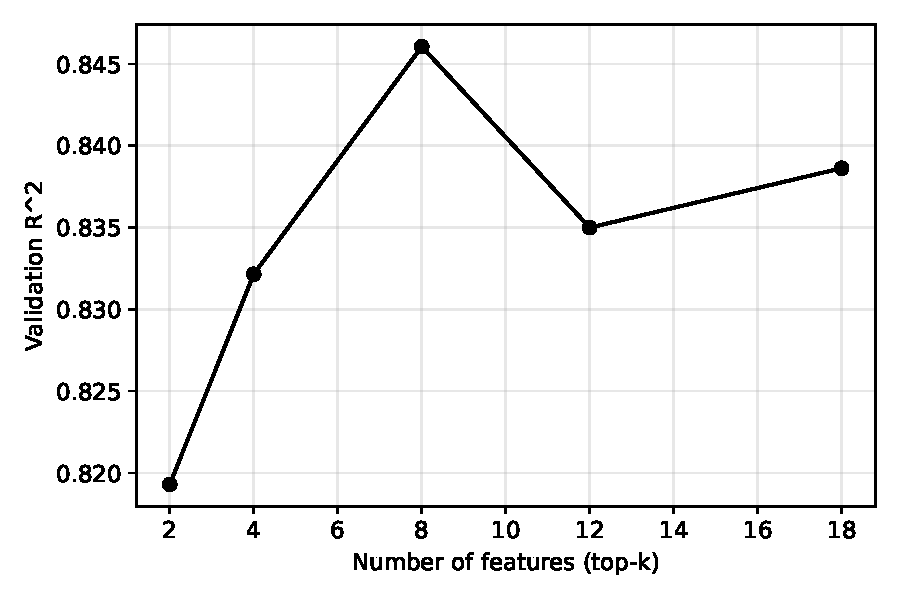
\includegraphics[width=0.62\textwidth]{figures/fig_ablation_curve.pdf}
  \Description{Line chart of validation R-squared versus number of top-ranked
  features used, for k equals 2, 4, 8, 12, and 18. The curve rises sharply then
  peaks at k equals 8 before slightly dipping and recovering.}
  \caption{Ablation: validation $R^2$ of SELENE retrained on the top-$k$
  permutation features. The curve shows how quickly predictive skill saturates as
  informative features are added.}
  \label{fig:ablation}
\end{figure}

Table~\ref{tab:ablation} reports all four metrics (Eqs.~\ref{eq:mse-mae}--
\ref{eq:mape}) at each $k$, not just $R^2$. MAPE, which weights
relative error and is therefore most sensitive to the low-dose majority of days
(Sect.~\ref{sec:dataset-stats}), is minimized at $k=12$ ($16.33\%$), one step
later than the $R^2$ optimum at $k=8$ ($R^2=0.846$), indicating a small
divergence between ``best average fit'' and ``best relative accuracy on typical
days'' that is worth keeping in mind when choosing a deployed feature set.

\begin{table}[t]
  \caption{Ablation: SELENE retrained on the top-$k$ permutation features, all
  four metrics (Eqs.~\ref{eq:mse-mae}--\ref{eq:mape}) on the validation
  set.}
  \label{tab:ablation}
  \begin{tabular}{p{1cm}p{2cm}p{2cm}p{1.8cm}p{1.8cm}}
    \hline\noalign{\smallskip}
    $k$ & MSE & MAE & $R^2$ & MAPE \\
    \noalign{\smallskip}\svhline\noalign{\smallskip}
    2  & $0.001020$ & $0.004965$ & $0.8193$ & $19.43\%$ \\
    4  & $0.000948$ & $0.004612$ & $0.8321$ & $17.14\%$ \\
    8  & $0.000869$ & $0.004524$ & $\mathbf{0.8461}$ & $16.88\%$ \\
    12 & $0.000932$ & $0.004461$ & $0.8350$ & $\mathbf{16.33\%}$ \\
    18 & $0.000911$ & $0.004673$ & $0.8386$ & $17.18\%$ \\
    \noalign{\smallskip}\hline
  \end{tabular}
\end{table}

\subsection{Physical Interpretation}
The dominant features can be read against radiation physics. Both leading
features, \texttt{sis\_cnt\_C\_2} and \texttt{sis\_cnt\_O\_2}, are SIS-measured
solar-energetic-particle counts of carbon and oxygen, consistent with the fact
that SEP fluences, not the comparatively steady GCR background, drive the
large, transient dose enhancements that dominate day-to-day variance in the
target. That two independent, principled attribution methods (permutation
importance and SHAP) agree exactly on this ranking, while a structurally
different model (gradient-boosted trees) confirms \texttt{sis\_cnt\_C\_2} as the
top feature, is strong evidence that SELENE has learned a physically meaningful
mapping rather than a spurious correlation. The one disagreement, XGBoost's
elevated weight on \texttt{ace\_cnt\_Ca\_5} and \texttt{ace\_cnt\_Fe\_4} (both GCR
heavy-ion channels from CRIS), most likely reflects tree ensembles' sensitivity
to rare, high-leverage GCR spikes that shuffling-based permutation importance
and SHAP's background-sample averaging tend to smooth over, rather than a
genuine physical signal the neural network is missing.

% ====================================================================
\section{Calibrated Uncertainty for Operational Risk}
\label{sec:calib}

For a dose-rate model to support shelter or scheduling decisions, its stated
uncertainty must be meaningful: a nominal 90\% prediction interval should contain
the truth about 90\% of the time. We compare three uncertainty-quantification
strategies and assess their calibration.

\subsection{Methods}
\emph{Monte Carlo (MC) dropout} keeps dropout active at inference and performs
$T=100$ stochastic forward passes per input~\cite{gal2016dropout}. Writing
$f_t(x)$ for the model's output on pass $t$ (a different random dropout mask
each time), the predictive mean and variance are the empirical moments of the
sample,
\begin{equation}
  \mu(x) = \frac{1}{T}\sum_{t=1}^{T} f_t(x), \qquad
  \sigma^2(x) = \frac{1}{T}\sum_{t=1}^{T} \bigl(f_t(x) - \mu(x)\bigr)^2.
  \label{eq:mc-dropout}
\end{equation}
\emph{Deep ensembles} train $N=10$ independently initialized copies of SELENE,
$g_1,\dots,g_N$, each on the same training data but a different random seed, and
compute the identical moments (Eq.~\ref{eq:mc-dropout}) with $g_n(x)$ in
place of $f_t(x)$ and $N$ in place of
$T$~\cite{lakshminarayanan2017ensembles}. In both cases a $(1-\alpha)$ central
interval is $[\mu(x) - z_{\alpha/2}\,\sigma(x),\ \mu(x) + z_{\alpha/2}\,\sigma(x)]$
with $z_{0.05} \approx 1.645$ for our $90\%$ intervals.

\emph{Quantile regression} instead trains a separate network $h_q$ for each
target quantile $q \in \{0.05, 0.5, 0.95\}$ under the pinball
(quantile) loss~\cite{koenker1978regression,rasp2018neural},
\begin{equation}
  \mathcal{L}_q(y, \hat{y}) =
  \begin{cases}
    q\,(y - \hat{y}) & \text{if } y \ge \hat{y} \\
    (q-1)(y - \hat{y}) & \text{if } y < \hat{y},
  \end{cases}
  \label{eq:pinball}
\end{equation}
which is minimized when $\hat{y}$ equals the true $q$-quantile of $y \mid x$; the
$90\%$ interval is then directly $[h_{0.05}(x), h_{0.95}(x)]$, with no
sampling required.

We evaluate all three methods with three metrics on the validation set of size
$n_v$, given interval $[\ell_i, u_i]$ for sample $i$:
\begin{align}
  \mathrm{PICP} &= \frac{1}{n_v}\sum_{i=1}^{n_v} \mathbb{1}[\ell_i \le y_i \le u_i],
  \label{eq:picp} \\
  \mathrm{MPIW} &= \frac{1}{n_v}\sum_{i=1}^{n_v} (u_i - \ell_i),
  \label{eq:mpiw} \\
  \mathrm{ECE} &= \frac{1}{|P|}\sum_{p \in P}
    \bigl\lvert \widehat{\mathrm{cov}}(p) - p \bigr\rvert,
  \label{eq:ece}
\end{align}
where $\mathbb{1}[\cdot]$ is the indicator function, $P$ is a grid of $10$
nominal coverage levels from $5\%$ to $95\%$, and $\widehat{\mathrm{cov}}(p)$ is
the empirical fraction of validation samples whose true value falls within the
corresponding central interval at level $p$ (assuming Gaussian
$\mu,\sigma$ for MC dropout and the ensemble, and the symmetric proxy
$\sigma_q = (u_i - \ell_i)/(2z_{0.05})$ for quantile
regression)~\cite{guo2017calibration,kuleshov2018calibrated}. A perfectly
calibrated method has $\mathrm{PICP} = 0.90$ (for our $90\%$ intervals) and
$\mathrm{ECE} = 0$; $\mathrm{MPIW}$ measures sharpness, with lower values
preferred at equal calibration.

\subsection{Results}
Table~\ref{tab:calib} reports the three methods. Quantile regression achieved
the best calibration, with $\mathrm{ECE} = 0.174$ and $\mathrm{PICP} = 0.804$
against the nominal $0.90$, while the deep ensemble produced the narrowest
intervals ($\mathrm{MPIW} = 0.0038$) but the worst calibration
($\mathrm{ECE} = 0.345$) and coverage ($\mathrm{PICP} = 0.335$). MC dropout fell
between the two ($\mathrm{ECE} = 0.201$, $\mathrm{PICP} = 0.614$). The
reliability diagram (Figure~\ref{fig:reliability}) shows all three curves lying
below the diagonal at every nominal level: every method is
overconfident, with empirical coverage below nominal coverage. The deep
ensemble deviates most severely, while quantile regression tracks closest to the
ideal line. The calibration--sharpness view (Figure~\ref{fig:calibsharp}) makes
the trade-off explicit: the deep ensemble is markedly sharper (narrower
intervals) but at the cost of coverage that is unusable for a 90\% nominal
guarantee, whereas quantile regression sacrifices sharpness for intervals whose
stated confidence is far closer to being trustworthy.

\begin{table}[t]
  \caption{Uncertainty-quantification methods on the validation set. PICP is
  coverage of the nominal 90\% interval (target $0.90$); MPIW is mean interval
  width (sharpness, lower is better); ECE is expected calibration error (lower is
  better); RMSE is point-prediction error.}
  \label{tab:calib}
  \begin{tabular}{p{2.4cm}p{1.4cm}p{1.4cm}p{1.4cm}p{1.4cm}}
    \hline\noalign{\smallskip}
    Method & PICP & MPIW & ECE & RMSE \\
    \noalign{\smallskip}\svhline\noalign{\smallskip}
    MC dropout      & 0.614 & 0.0107 & 0.201 & 0.0328 \\
    Deep ensemble   & 0.335 & 0.0038 & 0.345 & 0.0305 \\
    Quantile reg.\  & 0.804 & 0.1001 & 0.174 & 0.0636 \\
    \noalign{\smallskip}\hline
  \end{tabular}
\end{table}

\begin{figure}[t]
  \centering
  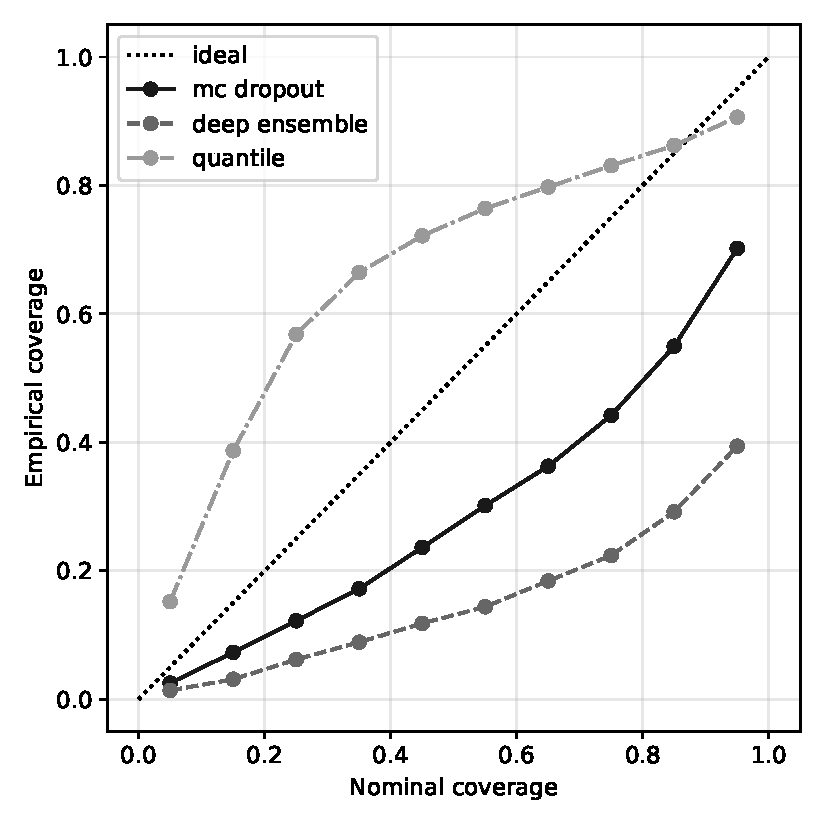
\includegraphics[width=0.6\textwidth]{figures/fig_reliability.pdf}
  \Description{Reliability diagram with nominal coverage on the horizontal
  axis and empirical coverage on the vertical axis. A diagonal dotted line
  marks perfect calibration; all three method curves fall below it, with the
  deep-ensemble curve farthest below and the quantile-regression curve
  closest.}
  \caption{Reliability diagram: empirical vs.\ nominal central-interval coverage
  for the three methods. Curves on the diagonal are perfectly calibrated; curves
  below it are over-confident.}
  \label{fig:reliability}
\end{figure}

\begin{figure}[t]
  \centering
  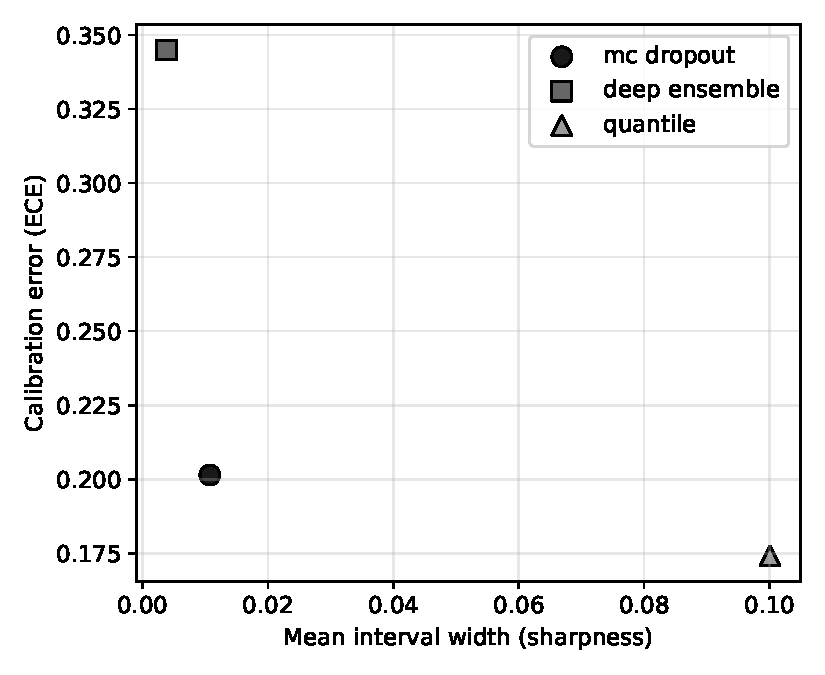
\includegraphics[width=0.6\textwidth]{figures/fig_calibration_sharpness.pdf}
  \Description{Scatter plot with mean interval width on the horizontal axis
  and expected calibration error on the vertical axis, one marker per method.
  The deep-ensemble marker sits at low width but high error; the
  quantile-regression marker sits at higher width but lower error.}
  \caption{Calibration vs.\ sharpness: expected calibration error against mean
  interval width. The preferred region is the lower left (well calibrated and
  sharp).}
  \label{fig:calibsharp}
\end{figure}

\subsection{Operational Risk Flagging}
Calibrated uncertainty enables a simple operational rule: flag a prediction as
low-confidence when its estimated interval width (or predictive variance) exceeds
a threshold, prompting an operator to fall back on a conservative physics-based
estimate or to defer an activity. Because quantile regression is the
best-calibrated method, we recommend deriving the flag from its predicted
interval width, with the threshold set at the 90th percentile of validation
interval widths (i.e., flagging the widest 10\% of predicted intervals). Even
under this best-calibrated method, empirical coverage ($0.804$) still falls
short of the nominal $0.90$, meaning the true dose lies outside the stated
90\% interval more often than intended; operators should therefore treat
quantile regression's intervals as a lower bound on uncertainty rather than an
exact guarantee, and treat any flagged (wide-interval) prediction, together with
any prediction near the top of the observed dose range, as warranting a
conservative fallback. This turns the model's imperfect but still informative
uncertainty into an actionable, if conservative, safety signal.

\subsection{A Worked Example}
Concretely, consider an operator monitoring the dose-rate nowcast during an
ongoing SEP event. Suppose quantile regression returns a median prediction
$\hat{y}_{0.5}$ with a 90\% interval $[\hat{y}_{0.05}, \hat{y}_{0.95}]$ whose
width places it in the top decile of validation interval widths, the flagging
condition defined above. Given the observed coverage gap
(Sect.~\ref{sec:calib}: $\mathrm{PICP} = 0.804$ against a nominal $0.90$), the
appropriate operational response is \emph{not} to treat $[\hat{y}_{0.05},
\hat{y}_{0.95}]$ as a strict 90\% guarantee, but to read the flag as a directive
to consult a physics-based estimate (e.g., from HZETRN or
REDMoon~\cite{Slaba2013,2022cosp...44.2697D}) before deciding whether the
predicted dose rate is high enough, relative to the mission's remaining
career-dose budget (Sect.~\ref{sec:background}), to warrant sheltering. In
this way the calibration analysis does not just characterize model quality in
the abstract; it directly determines how conservatively the flag must be
interpreted at the point of use.

% ====================================================================
\section{Discussion}
\label{sec:discussion}

The interpretability analysis shows that SELENE's
predictions rest on a small set of physically sensible ion/energy-band features
rather than on spurious correlations, and the ablation quantifies how much signal
each contributes. The calibration analysis shows that quantile regression
yields the prediction intervals whose stated confidence is most (though still
imperfectly) trustworthy, and provides a concrete rule for flagging
low-confidence predictions.
An operator equipped with both an interpretable attribution and a calibrated
confidence estimate is in a far stronger position to act on a nowcast than one
given a bare point prediction.

Several limitations qualify these findings. The dataset remains noisy and is
dominated by lower dose rates, so uncertainty is largest, and calibration hardest,
precisely in the high-dose regime that matters most operationally; this is the
same regime in which the original error analysis found the largest
residuals~\cite{tummala2025selene}. The model is trained on ACE L1 measurements
and CRaTER orbital dose, so transfer to surface dose under specific shielding
geometries would require additional modeling. Finally, our uncertainty estimates
capture model and (via ensembles) some data uncertainty, but not systematic
instrument or aggregation error.

The systematic overconfidence observed across all three uncertainty-
quantification methods (Sect.~\ref{sec:calib}) is itself informative. Rather
than treating it as a dead end, it points to a concrete next step: post-hoc
recalibration, in which a held-out calibration set is used to learn a monotonic
correction from a method's raw predicted quantiles to empirically calibrated
ones~\cite{kuleshov2018calibrated}, in the spirit of temperature scaling for
classification~\cite{guo2017calibration}. Because such recalibration is applied
after training and does not alter the underlying point predictions, it could be
layered onto any of the three methods evaluated here at negligible additional
cost, and closing the observed coverage gap (Table~\ref{tab:calib}) is a natural
next milestone before operational deployment.

% ====================================================================
\section{Future Work and Conclusion}
\label{sec:conclusion}

\paragraph{Future work.}
Three directions follow naturally. First, \emph{temporal modeling}: incorporating
lagged fluxes and rolling statistics, and recurrent or convolutional
architectures, to capture the delayed and event-driven nature of SEP dose. Second,
\emph{calibrated high-dose specialization}: cost-sensitive or heavy-tailed losses
and post-hoc recalibration~\cite{kuleshov2018calibrated} targeted at the
operationally critical high-dose regime. Third, \emph{deployment and transfer}:
measuring inference cost for onboard use, and adapting the framework to the
Martian radiation environment, where analogous upstream measurements and surface
dosimetry are becoming available. A fourth, longer-horizon direction is
\emph{hybrid physics-ML modeling}: using SELENE as a fast first-pass estimator
that triggers a full HZETRN or GEANT4-based
calculation~\cite{Slaba2013,2022cosp...44.2697D} only when its own calibrated
uncertainty is high, combining the speed of the data-driven approach with the
physical fidelity of transport codes precisely where the neural model is least
confident; this architecture is made possible only once uncertainty is
calibrated, which is the contribution of Sect.~\ref{sec:calib}.

\paragraph{Conclusion.}
Fast machine-learning estimation of lunar radiation dose is
feasible~\cite{tummala2025selene}, but operational use demands more than speed and
accuracy. By equipping SELENE with physical interpretability and calibrated
uncertainty, this chapter converts a black-box regressor into a nowcasting tool
whose predictions can be explained and whose confidence can be trusted. These
properties, not accuracy alone, are what make a data-driven model usable for
protecting humans in the harsh radiation environment of the Moon, and they carry
directly toward the deeper-space missions that will follow.

\bibliographystyle{spmpsci}
\bibliography{references}

\end{document}
